% !TeX spellcheck = en_GB

%%%%%%%%%%%%%%%%%%%%%%%%%%%%%%%%%%%%%%%%%%%%%%%%%%%%%%%%%%%%%%%%%%%%%%%%%
%%%%%%%% large scale pheonmena vertical ? %%%%%%%%%%%%%%
\section{Observation of large scale weather phenomena in the vertical}
%%%%%%%%% image reflectivity %%%%%%%%%%%%%%
\begin{figure}[h!]
	\centering
    % 23/12
    \begin{subfigure}[t]{\textwidth}
    \centering
    	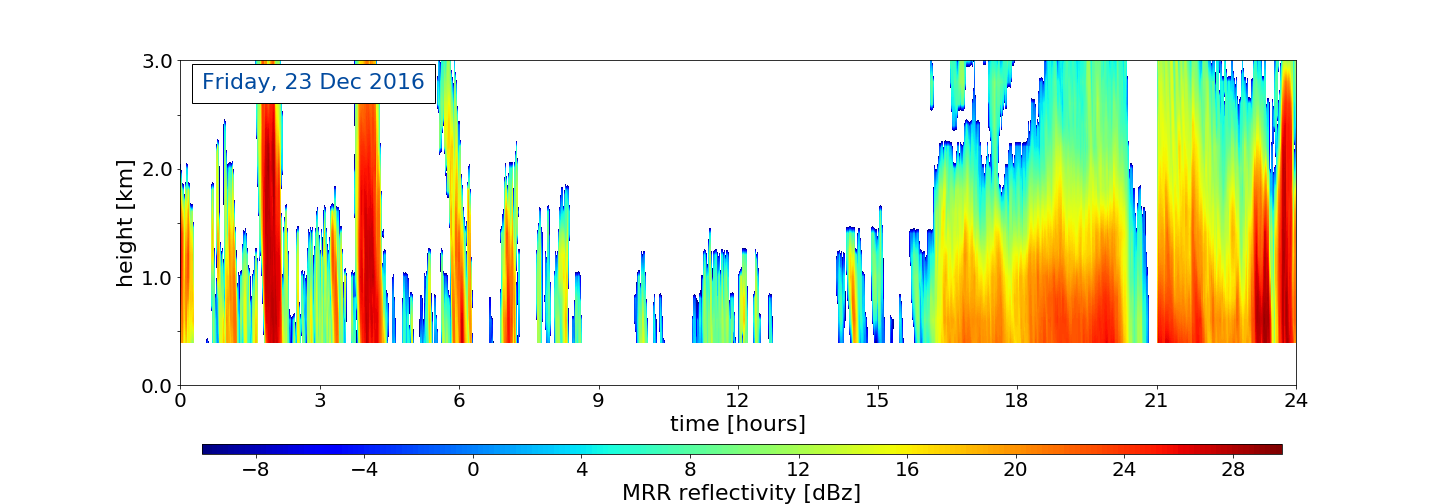
\includegraphics[trim={4.cm 2.5cm 4.5cm 1.5cm},clip,width=\textwidth]{./fig_MRR_refl/MRR_20161223}
		\caption{}\label{fig:ret:refl23}
    \end{subfigure}
    % 25/12
    \begin{subfigure}[t]{\textwidth}
    \centering
    	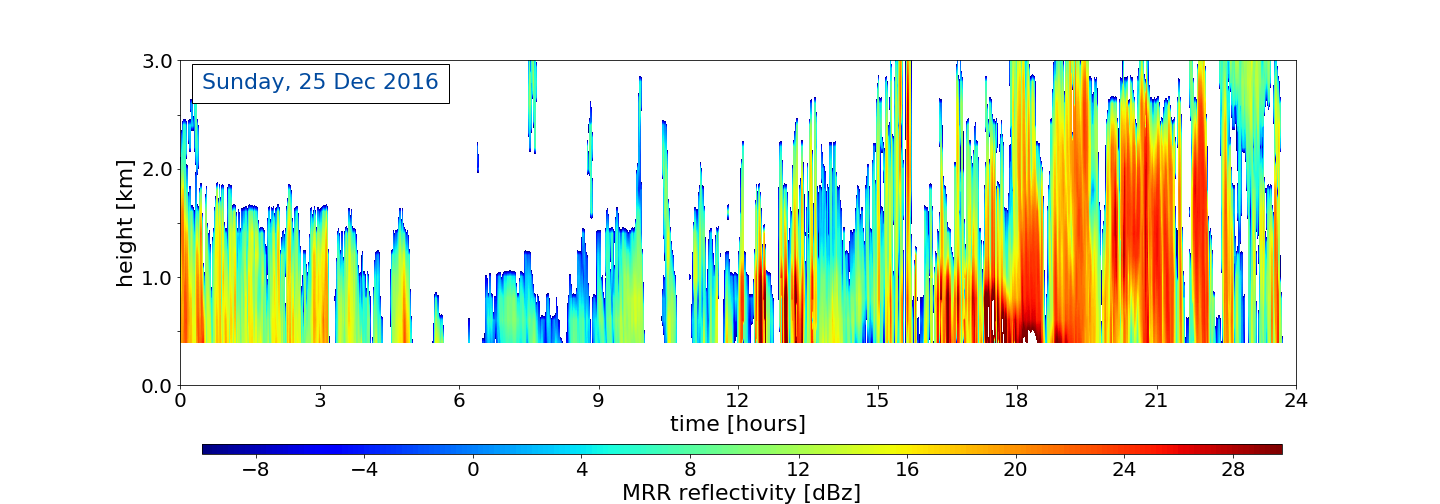
\includegraphics[trim={4.cm 2.5cm 4.5cm 1.5cm},clip,width=\textwidth]{./fig_MRR_refl/MRR_20161225}
		\caption{}\label{fig:ret:refl25}
    \end{subfigure}
    % 26/12
    \begin{subfigure}[t]{\textwidth}
    \centering
    	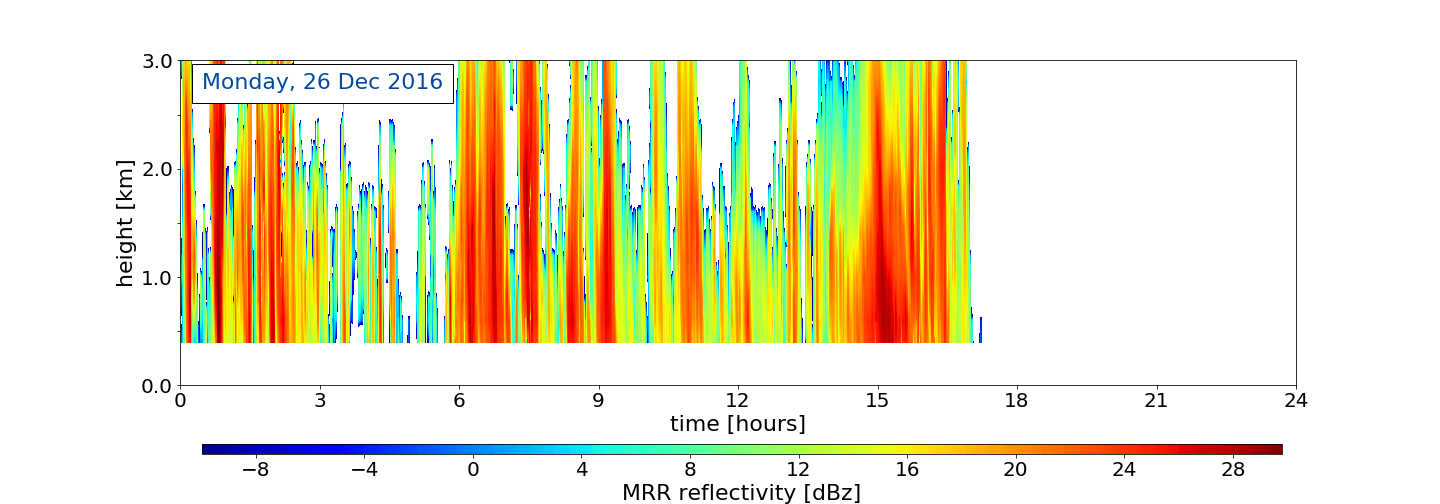
\includegraphics[trim={4.cm 2.5cm 4.5cm 1.5cm},clip,width=\textwidth]{./fig_MRR_refl/MRR_20161226}
		\caption{}\label{fig:ret:refl26}
    \end{subfigure}
    % label
    \begin{subfigure}[t]{\textwidth}
    	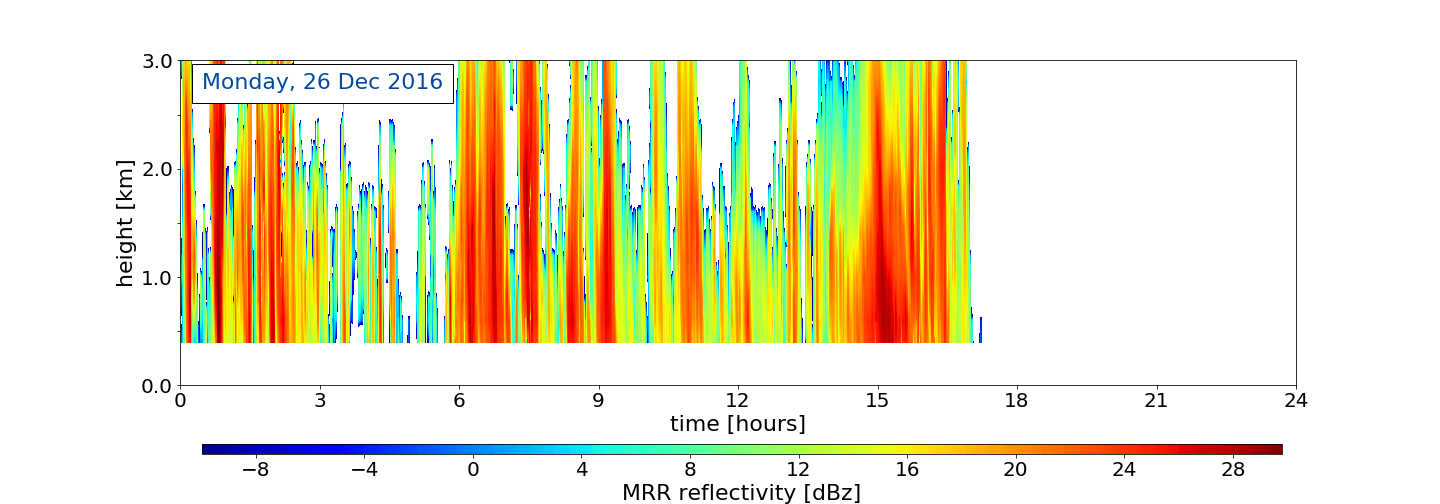
\includegraphics[trim={6.5cm 0cm 5.3cm 15.5cm},clip,width=\textwidth]{./fig_MRR_refl/MRR_20161226}
    \end{subfigure}
    \caption{MRR reflectivity for the days when a front or an occlusion passed through at Haukeliseter. \SI{}{\decibel Z} reflectivities according to the colour bar, with weaker precipitation in blue and more intense precipitation in red. \protect\subref{fig:ret:refl23}: Friday, \SI{23}{\dec}, \protect\subref{fig:ret:refl25}: Sunday, \SI{25}{\dec}, and \protect\subref{fig:ret:refl26}: Monday, \SI{26}{\dec}.}\label{fig:ret:refl}
\end{figure}
%%%%%%%%%%%%%%%%%%%%%%%%%%%%%%%%%%%%%%%%%%%%%%%%%%%%%%%%%%%%%%%%%%%%%%%%%
\noindent
\Cref{fig:ret:refl} shows the reflectivity from the MRR at Haukeliseter for \SIlist{23;25;26}{\dec}. Passages of occluded fronts and a warm sector were observed on \SIlist{23;25}{\dec} and \SI{26}{\dec}, respectively. \Cref{fig:ret:refl26} presents only values until \SI{17}{\UTC}, because the precipitation change followed that drops froze to the dish and the MRR signal got attenuated. 
\\
The transit of the boundaries shows in \Cref{fig:ret:refl} by the more consistent structure of a storm. While on \SIlist{23;25}{\dec} the reflectivity did not pass values larger than \SI{28}{\decibel Z} shows \Cref{fig:ret:refl25} high reflectivity values larger than \SI{30}{\decibel Z}. These high values indicate the observation of liquid precipitation, which was also observed by the MASC (\Cref{fig:res:obs_masc}). 
\\
On \SI{23}{\dec} let the surface observations assume that the occluded front passed through between \SIrange{12}{21}{\UTC} (\Cref{fig:res:sfc_pres23}). The vertical observations at Haukeliseter show intense reflectivity and therefore higher precipitation after \SI{16}{\UTC}. Another occlusion passed through on \SI{26}{\dec} shortly before \SI{15}{\UTC} until \SI{21}{\UTC}. The high reflectivity on both days shows the passage of the fronts. While the wind on \SI{23}{\dec} was from the south (\Cref{fig:res:sfc_temp23}) was the wind on \SI{25}{\dec} continues from the west. 
%%%%%%%%% image SWC retrieval MEPS 23 %%%%%%%%%%%%%%
\begin{figure}[t]
	\centering
    % 23/12
    \begin{subfigure}[t]{\textwidth}
    \centering
    	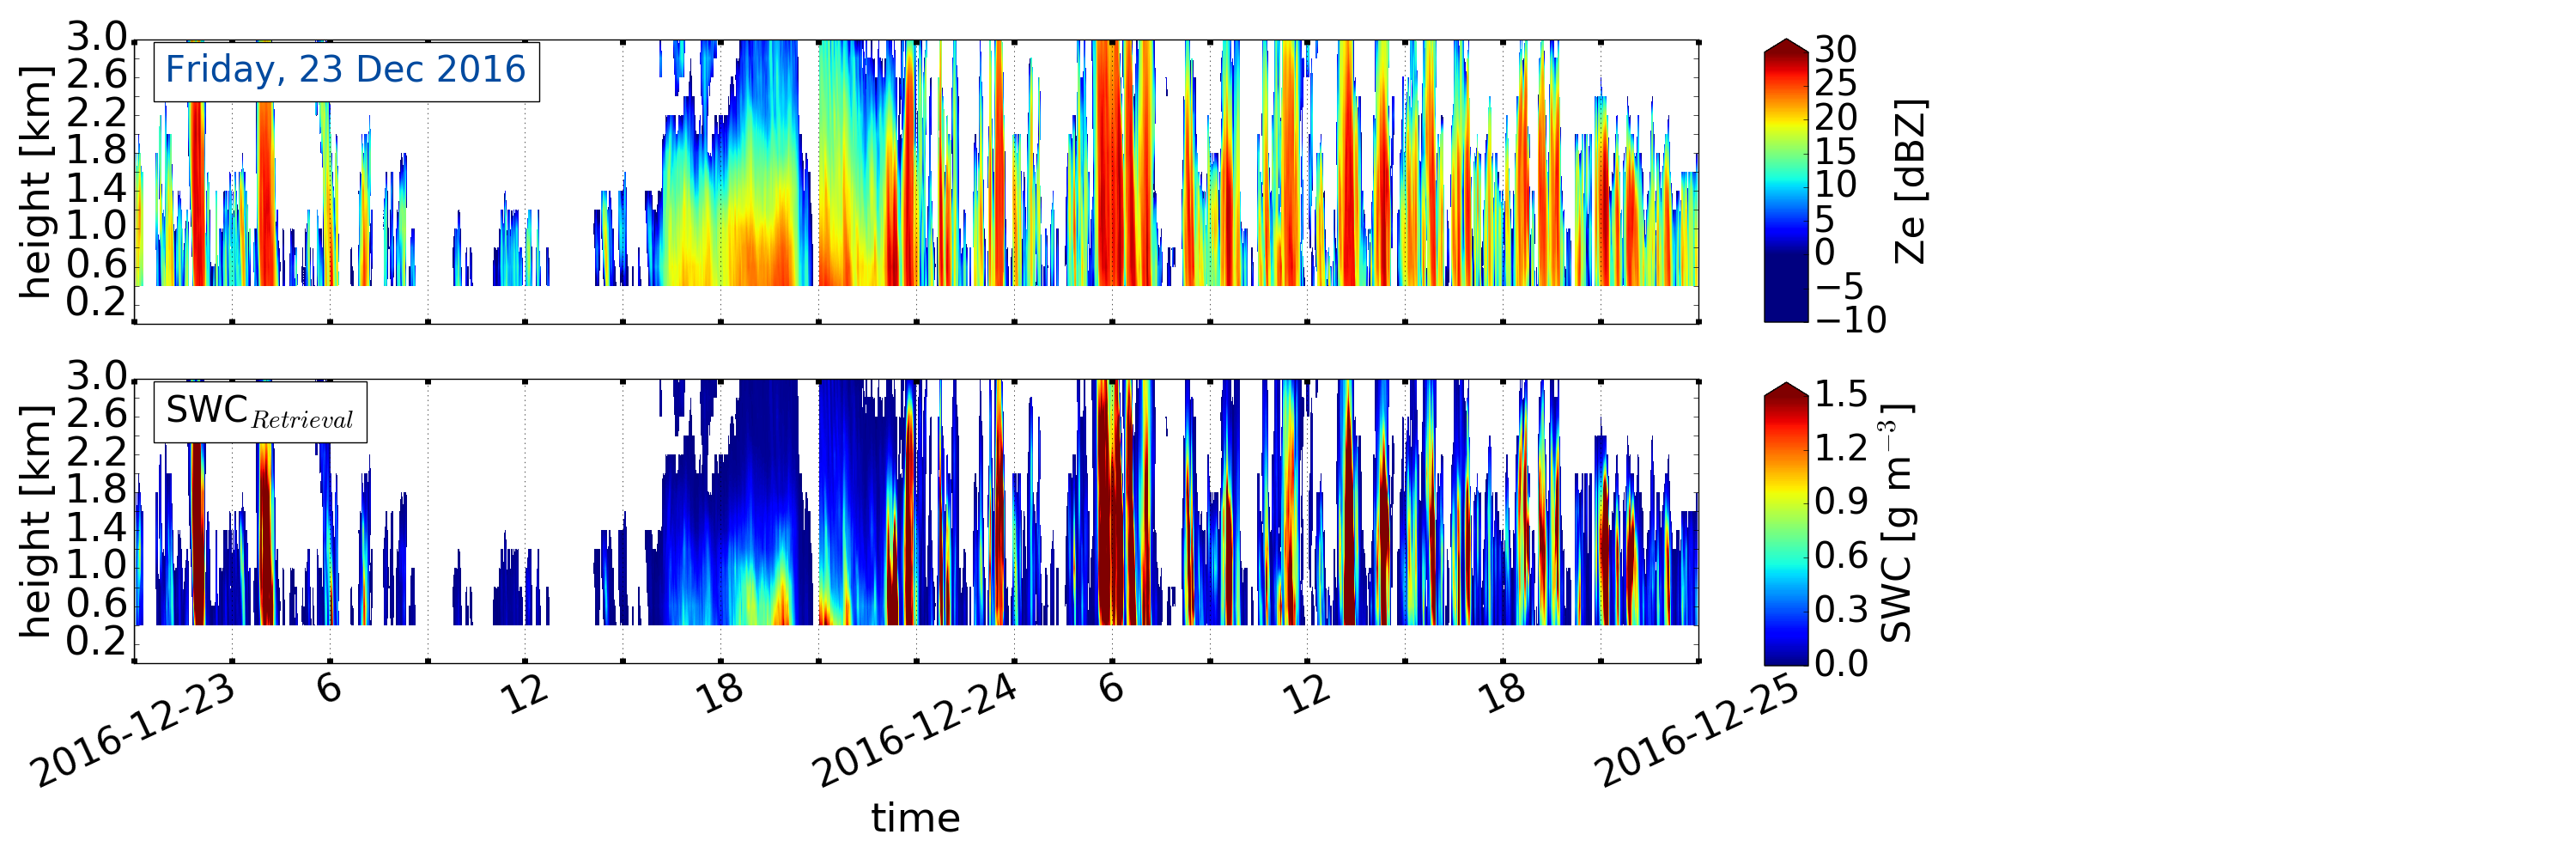
\includegraphics[trim={0.cm 2.2cm 19.cm 0.5cm},clip,width=0.9\textwidth]{./fig_obs_ret/20161223}
		\caption{}\label{fig:SWC:ret_23}
    \end{subfigure}
    % EM
    \begin{subfigure}[t]{\textwidth}
    \centering
    	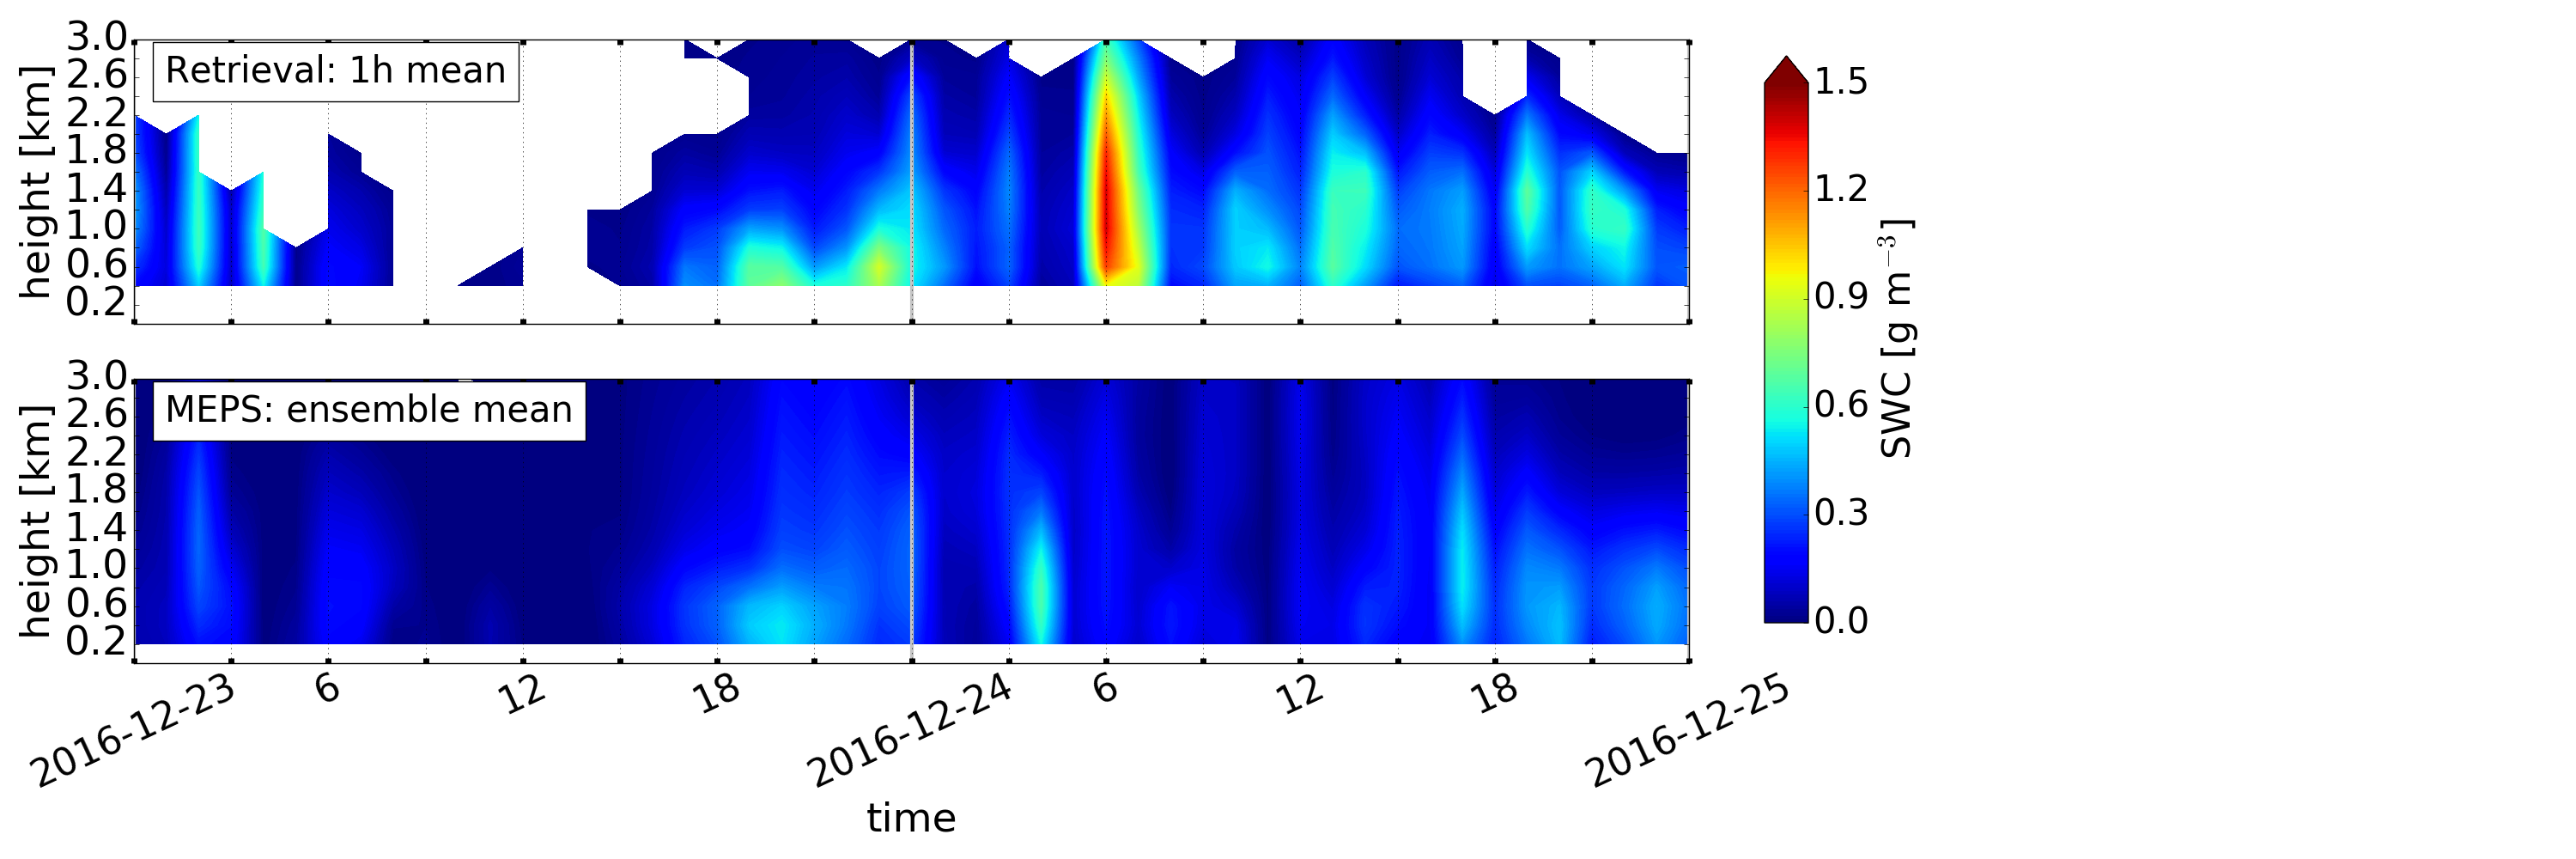
\includegraphics[trim={0.cm 2.2cm 19.cm 0.5cm},clip,width=0.9\textwidth]{./fig_vert_SWC_EM/20161223}
		\caption{}\label{fig:SWC_EM:23}
    \end{subfigure}
    % 3h
    \begin{subfigure}[t]{\textwidth}
    \centering
    	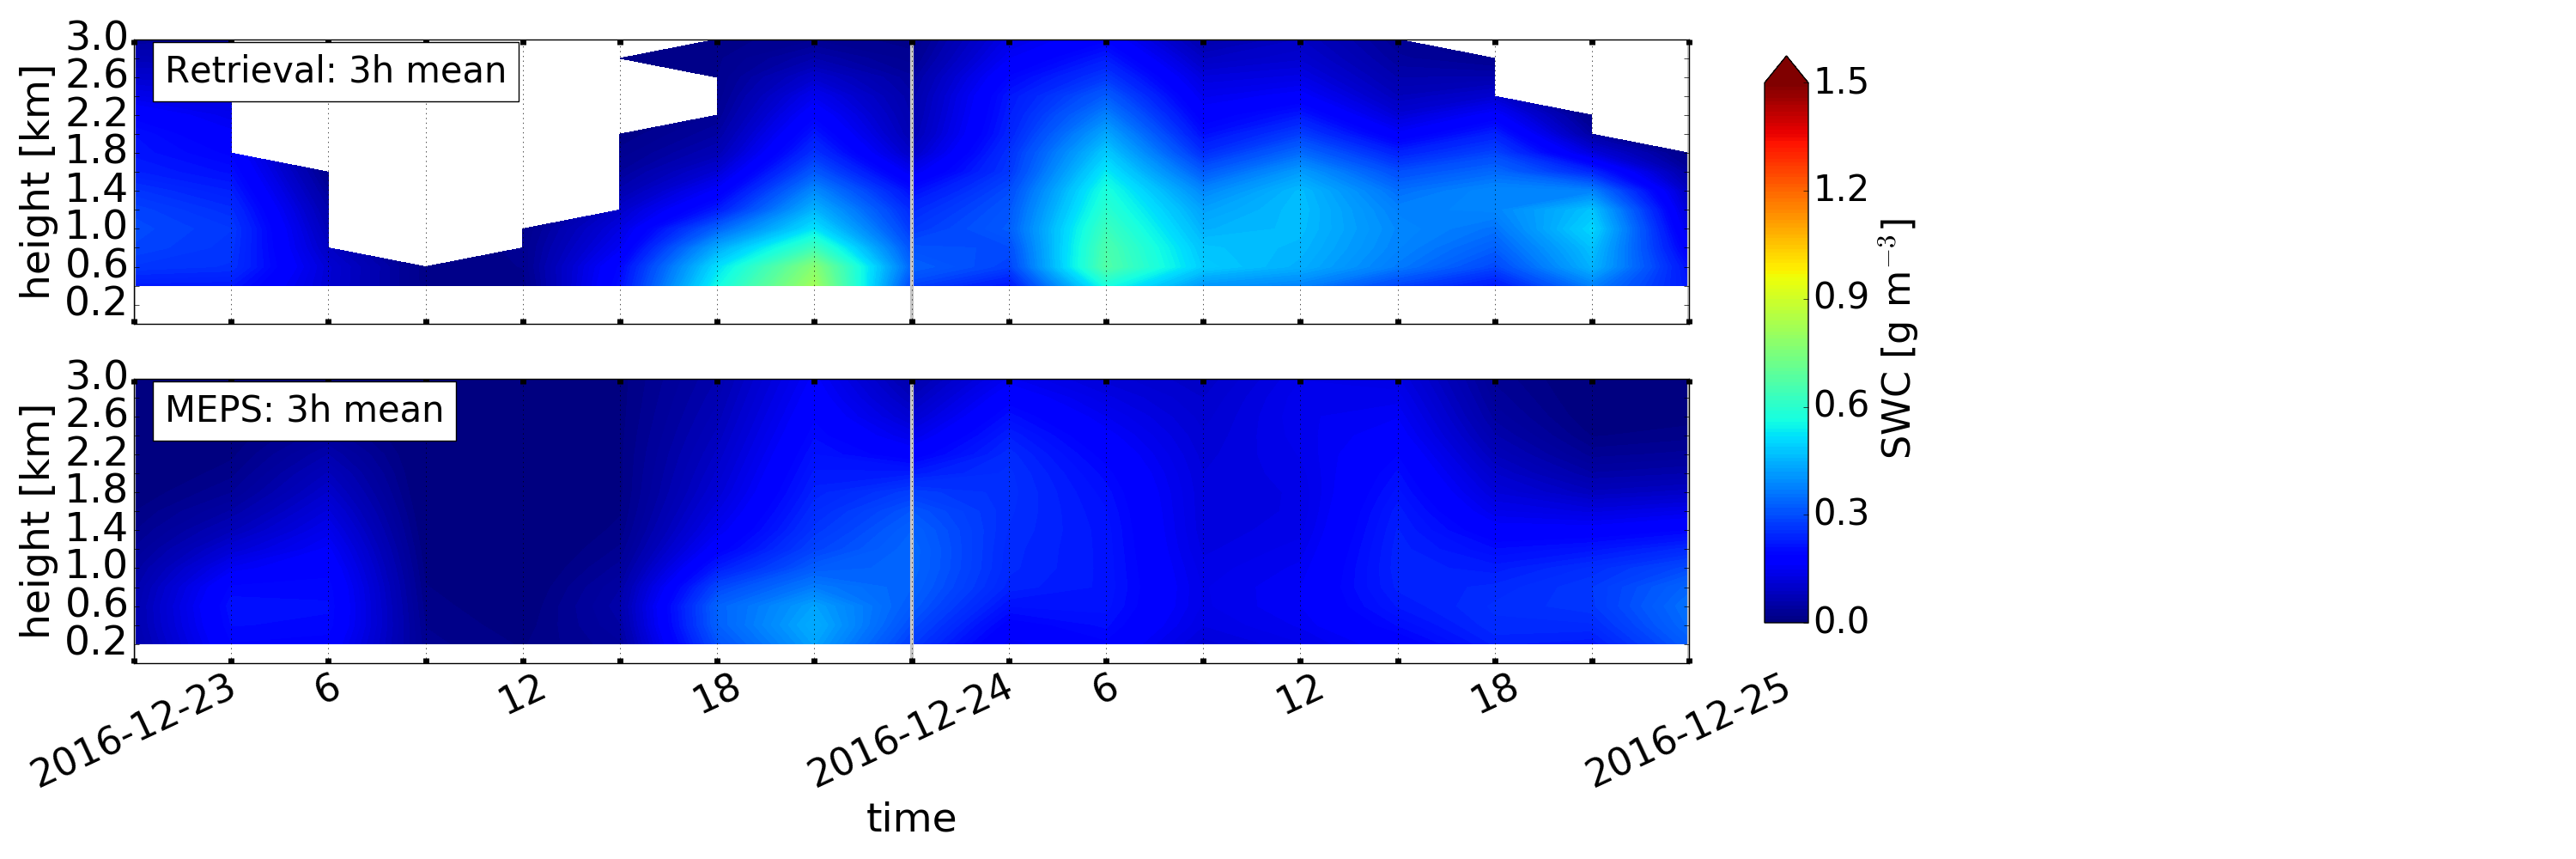
\includegraphics[trim={0.cm 0.8cm 19.cm 0.5cm},clip,width=0.9\textwidth]{./fig_vert_SWC_3h/20161223}
		\caption{}\label{fig:SWC3h:23}
    \end{subfigure}
 %   \caption{Initialisation \SI{23}{\dec} \SI{0}{\UTC}. \protect\subref{fig:SWC:ret_23}: upper panel MRR reflectivity for \SI{48}{\hour}, lower panel minutely retrieved SWC. \protect\subref{fig:SWC_EM:23}: upper panel hourly averaged retrieved SWC, lower panel instantaneous hourly averaged forecast of all ensemble member SWC, neglecting missing values. \protect\subref{fig:SWC3h:23}: upper panel three hourly averaged retrieved SWC, lower panel instantaneous three hourly averaged forecast of all ensemble member SWC.   }\label{fig:ret:SWC}
\end{figure}
%%%%%%%%%%%%%%%%%%%%%%%%%%%%%%%%%%%%%%%%%%%%%%%%%%%%%%%%%%%%%%%%%%%%%%%%%
The one hourly averaged values over all ensemble members in \Cref{fig:SWC_EM:23}, neglecting not existing values show, the consistent storm pattern after \SI{16}{\UTC}. Even the three hourly averaged values show the response. In general are the forecasted instantaneous snow water content weaker than the retrieved values for this time. Hourly averages, only using the deterministic forecast and the first ensemble member show no occurrence of the occlusion passage on either days. The variation of each ensemble members initialised on the respective day are given in \Cref{fig:EM09}. It shows that on \SI{23}{\dec} the first perturbed ensemble member does not exist and therefore little snow water content is predicted. By comparing to \SIlist{25;26}{\dec} it shows not much more snow water content is predicted when using the instantaneous values at every hour from the deterministic and first perturbed forecast. 
\\ 
On \SI{26}{\dec} when the passage of the occlusion is predicted, the three hourly instantaneous SWC (\Cref{fig:SWC3h:26}) as well as the average of all ensemble members (\Cref{fig:SWC_EM:26}) predict the frontal passage. The variation of all members in \Cref{fig:EM09_26} indicates that around \SI{16}{\UTC} almost all perturbed members would have predicted the precipiation. The deterministic forecast shows the highest SWC vales when comparing to the perturbed members, but in \Cref{fig:SWC1h:26} the amount of snow water content is very weak. It shows, that the ensemble mean of all members or with a course time resolution gives a better result than by only comparing the deterministic and the first perturbed member. Still the instantaneous average values of the ensemble members are much weaker than the retrieved SWC.
%%%%%%%%% image SWC retrieval MEPS 25 %%%%%%%%%%%%%%
\begin{figure}[t]\ContinuedFloat
	\centering
    % 25/12
    \begin{subfigure}[t]{\textwidth}
    \centering
    	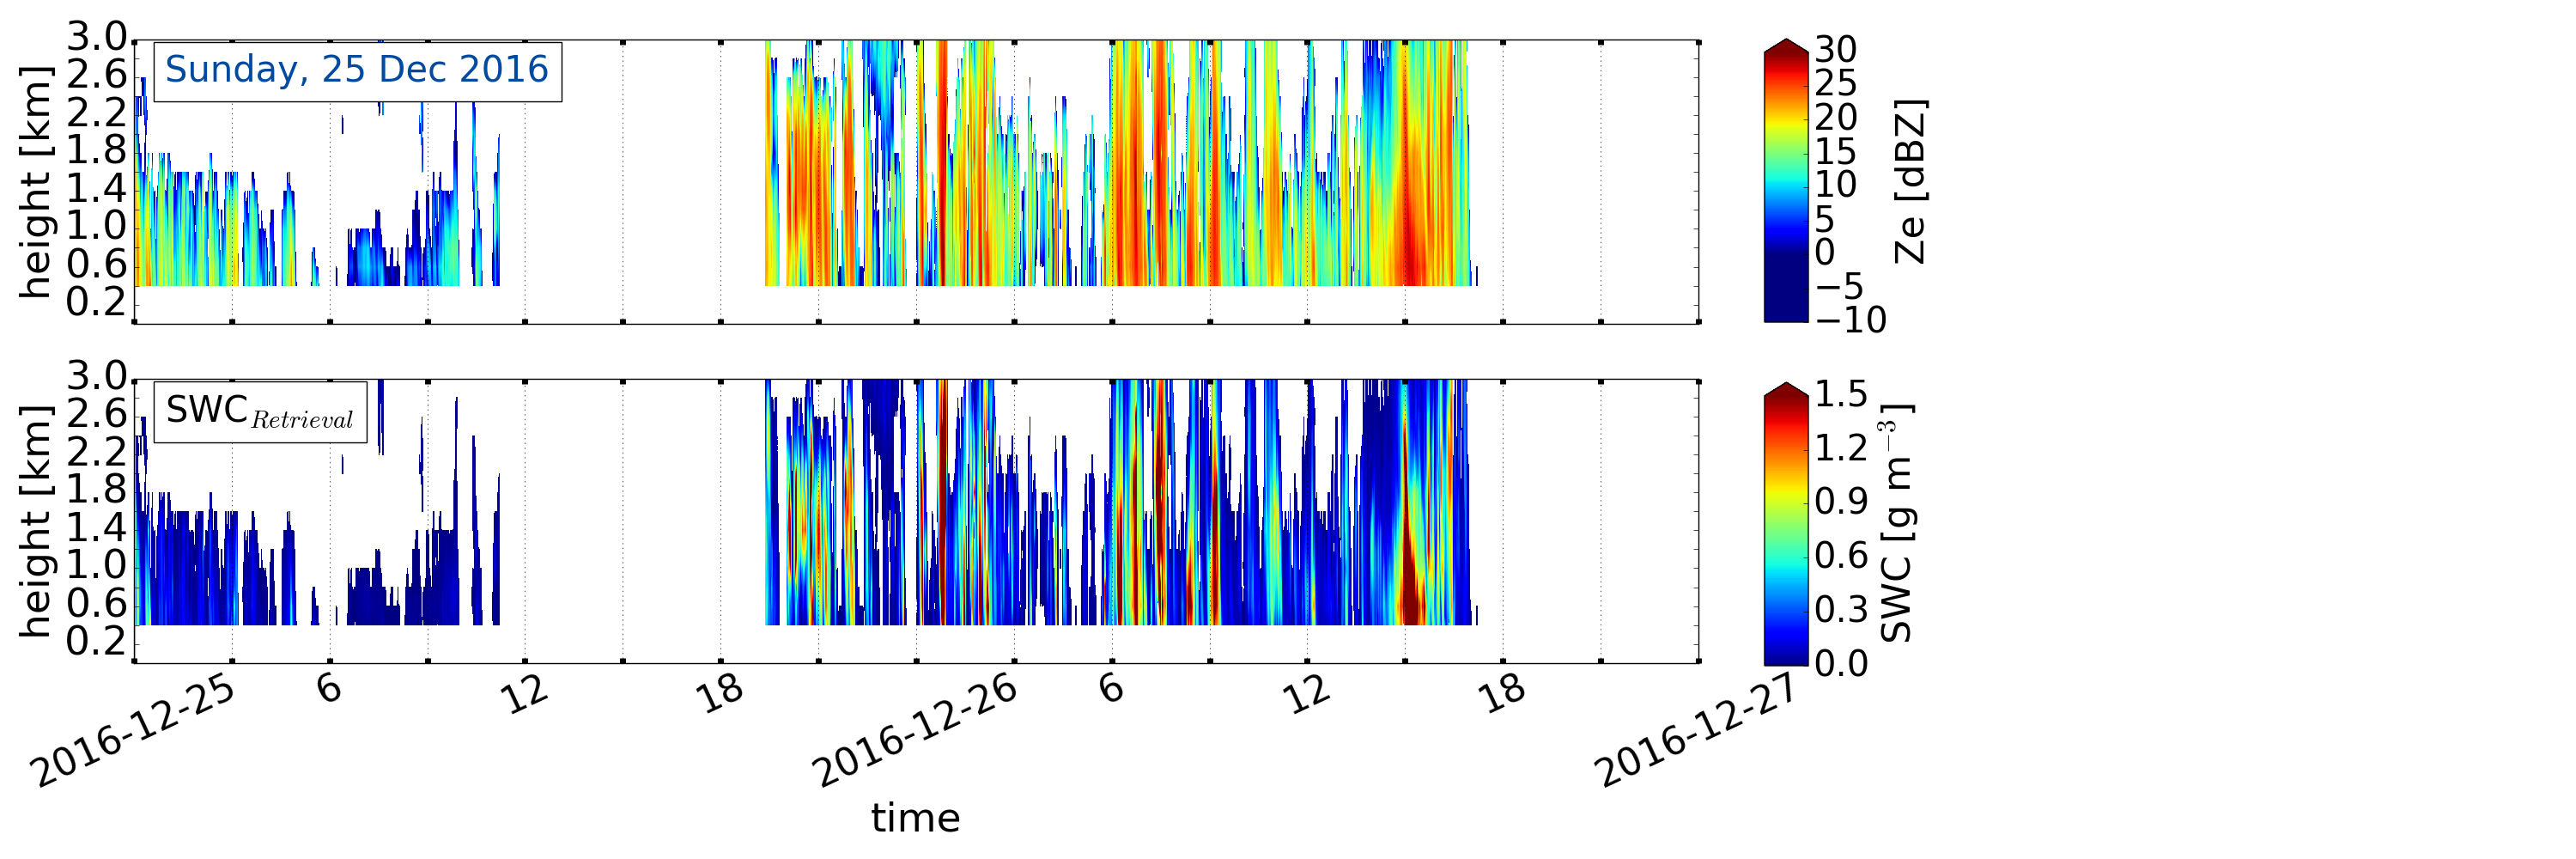
\includegraphics[trim={0.cm 2.2cm 19.cm 0.5cm},clip,width=0.9\textwidth]{./fig_obs_ret/20161225}
		\caption{}\label{fig:SWC:ret_25}
    \end{subfigure}
    % EM
    \begin{subfigure}[t]{\textwidth}
    \centering
    	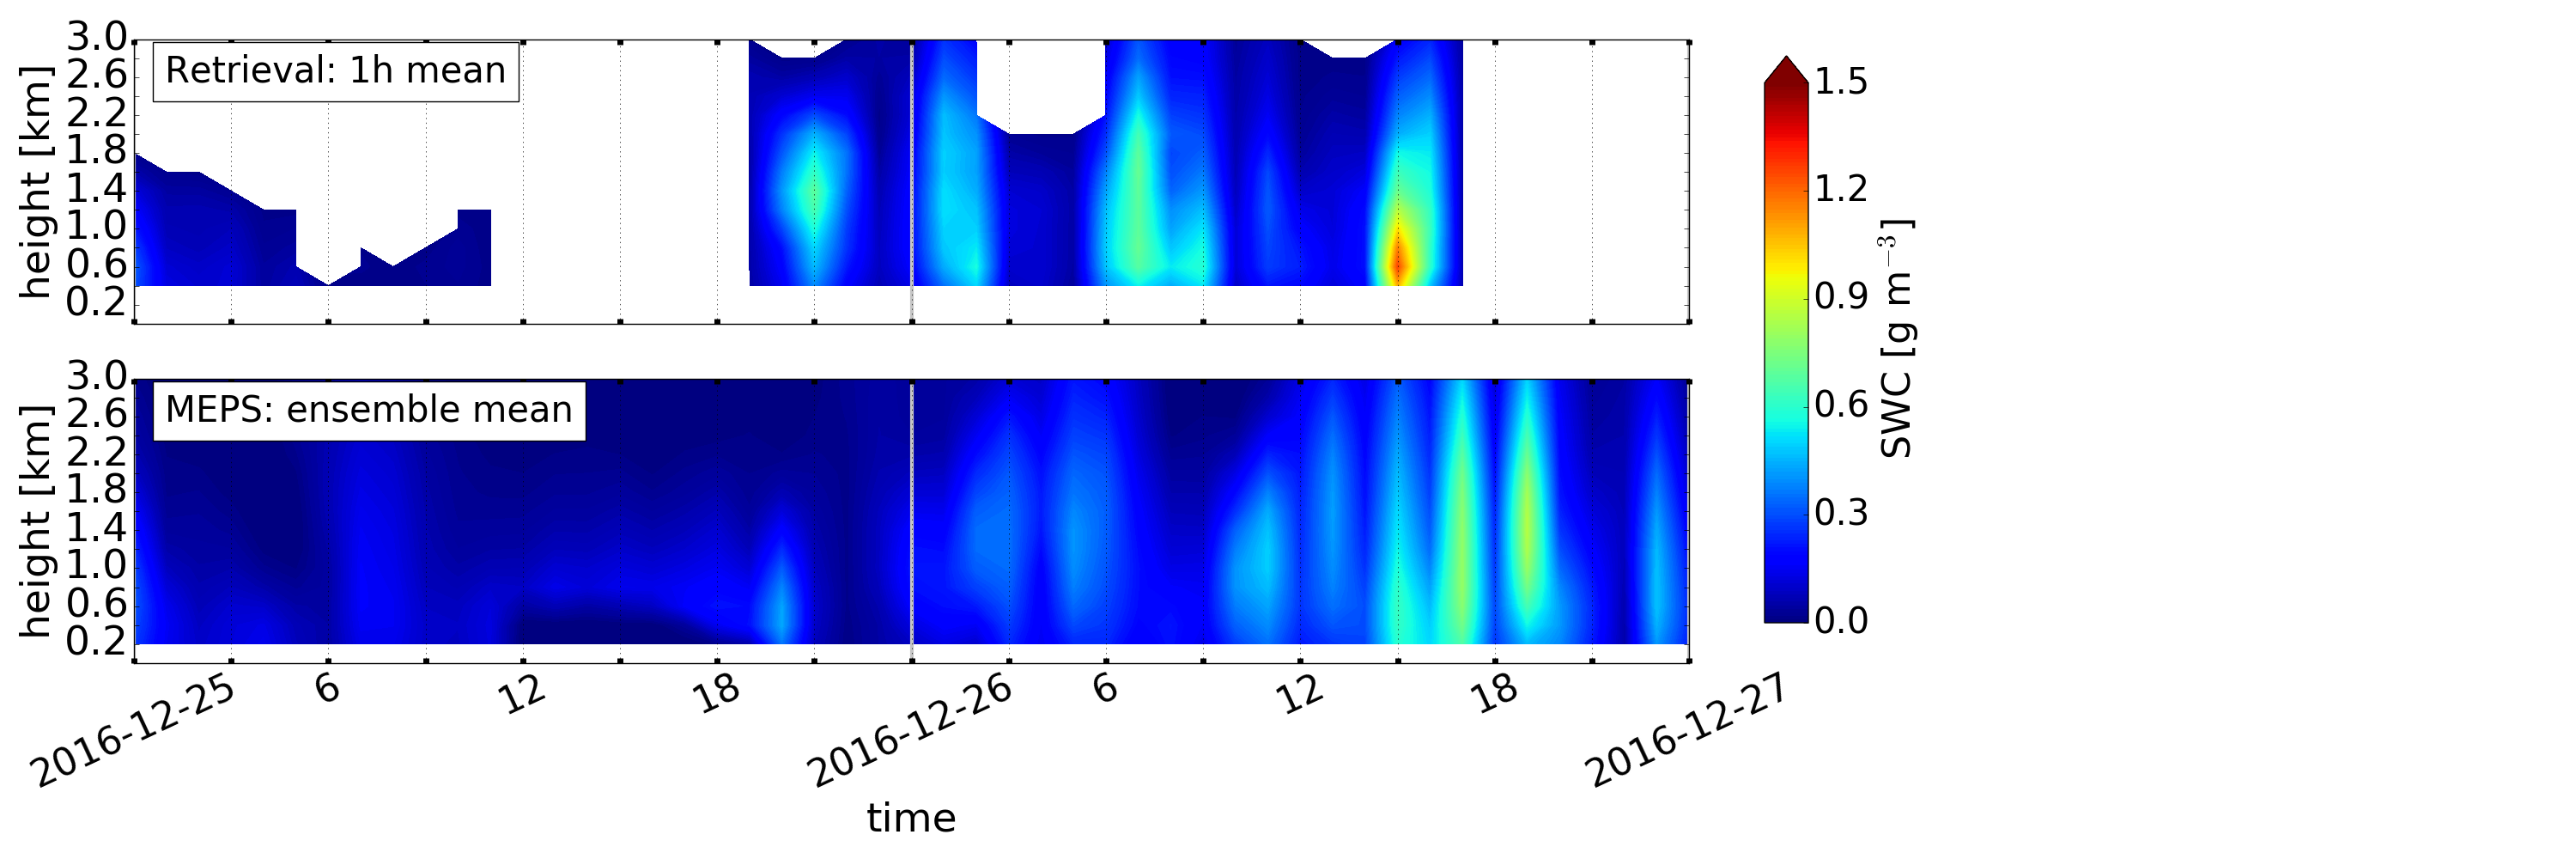
\includegraphics[trim={0.cm 2.2cm 19.cm 0.5cm},clip,width=0.9\textwidth]{./fig_vert_SWC_EM/20161225}
		\caption{}\label{fig:SWC_EM:25}
    \end{subfigure}
    % 3h
    \begin{subfigure}[t]{\textwidth}
    \centering
    	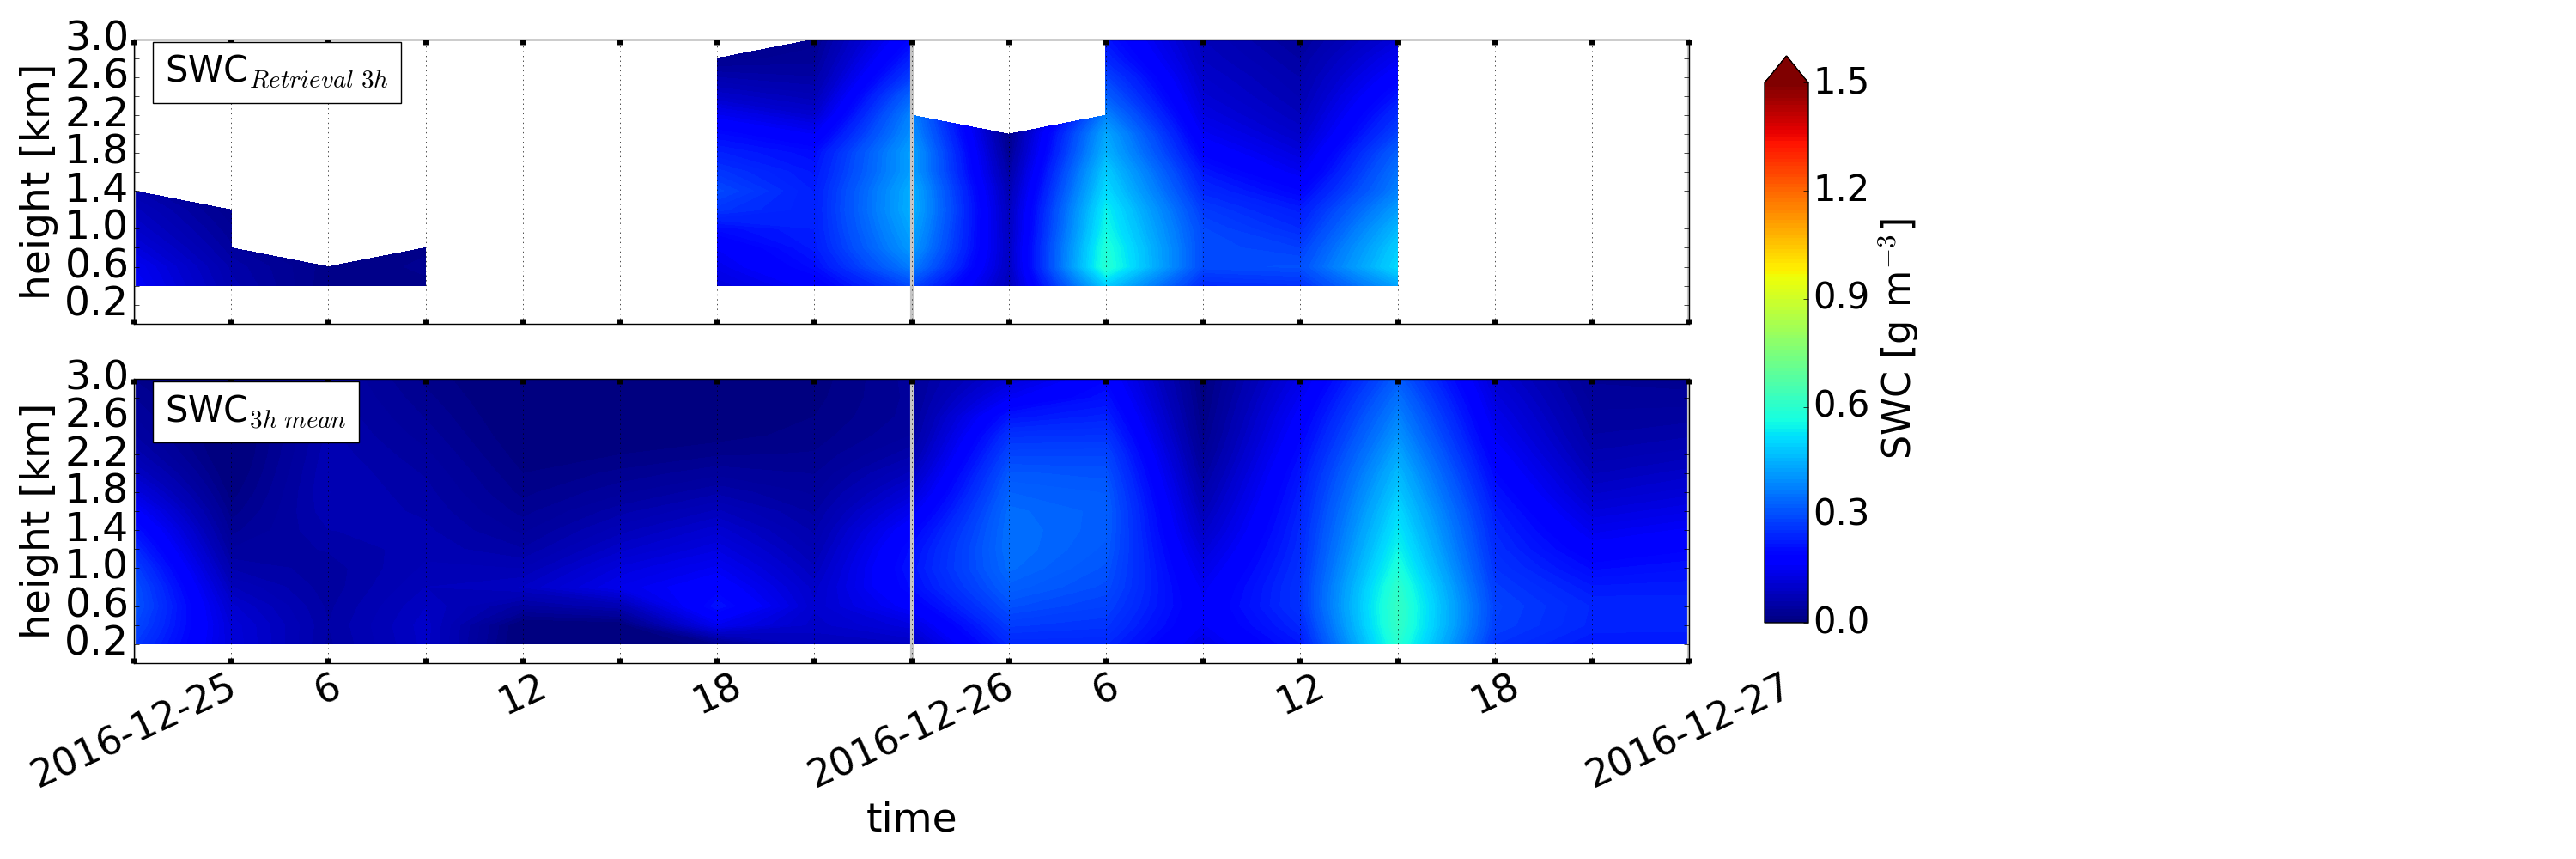
\includegraphics[trim={0.cm 0.8cm 19.cm 0.5cm},clip,width=0.9\textwidth]{./fig_vert_SWC_3h/20161225}
		\caption{}\label{fig:SWC3h:25}
    \end{subfigure}
\end{figure}
%%%%%%%%%%%%%%%%%%%%%%%%%%%%%%%%%%%%%%%%%%%%%%%%%%%%%%%%%%%%%%%%%%%%%%%%%
%%%%%%%%% image SWC retrieval MEPS 26 %%%%%%%%%%%%%%
\begin{figure}[t]\ContinuedFloat
	\centering
    % 25/12
    \begin{subfigure}[t]{\textwidth}
    \centering
    	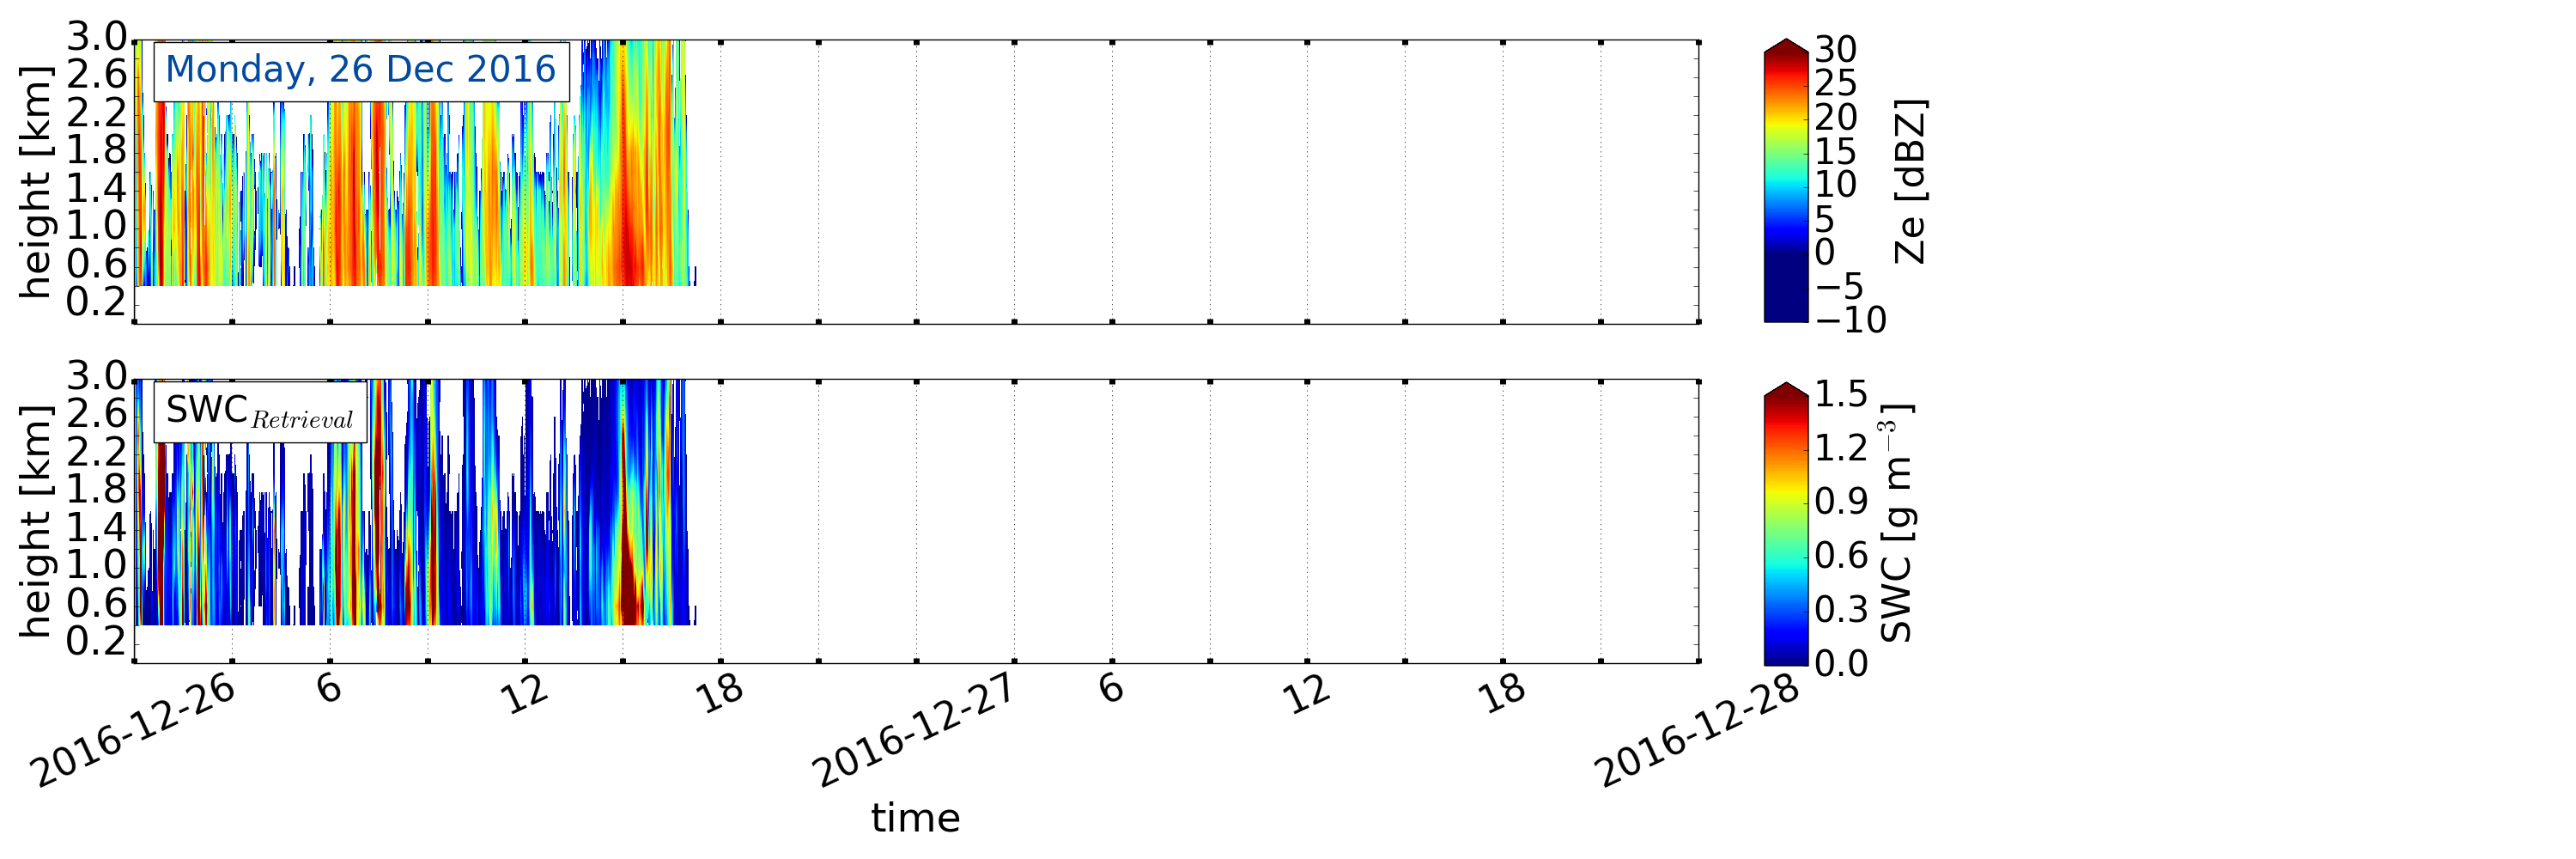
\includegraphics[trim={0.cm 2.2cm 19.cm 0.5cm},clip,width=0.9\textwidth]{./fig_obs_ret/20161226}
		\caption{}\label{fig:SWC:ret_26}
    \end{subfigure}
    % EM
    \begin{subfigure}[t]{\textwidth}
    \centering
    	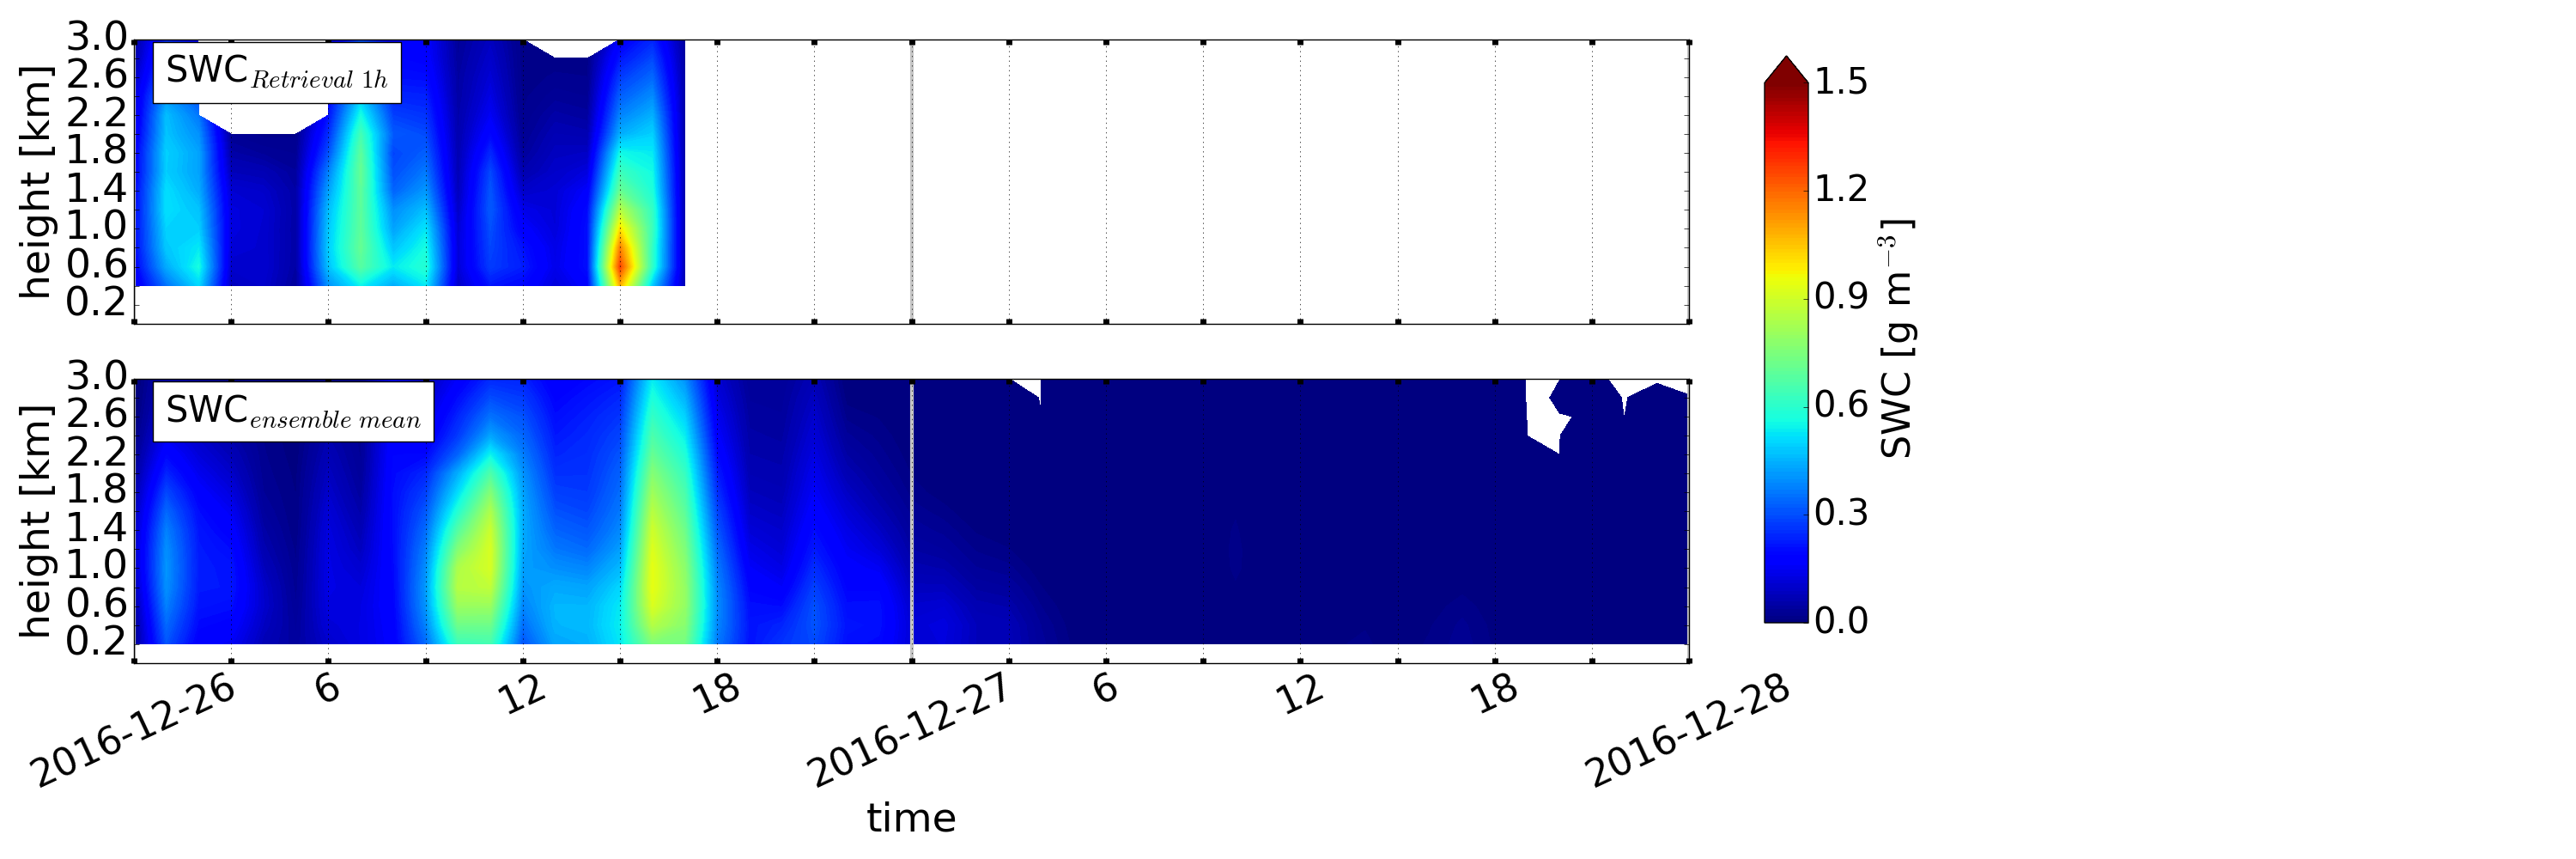
\includegraphics[trim={0.cm 2.2cm 19.cm 0.5cm},clip,width=0.9\textwidth]{./fig_vert_SWC_EM/20161226}
		\caption{}\label{fig:SWC_EM:26}
    \end{subfigure}
    % 3h
    \begin{subfigure}[t]{\textwidth}
    \centering
    	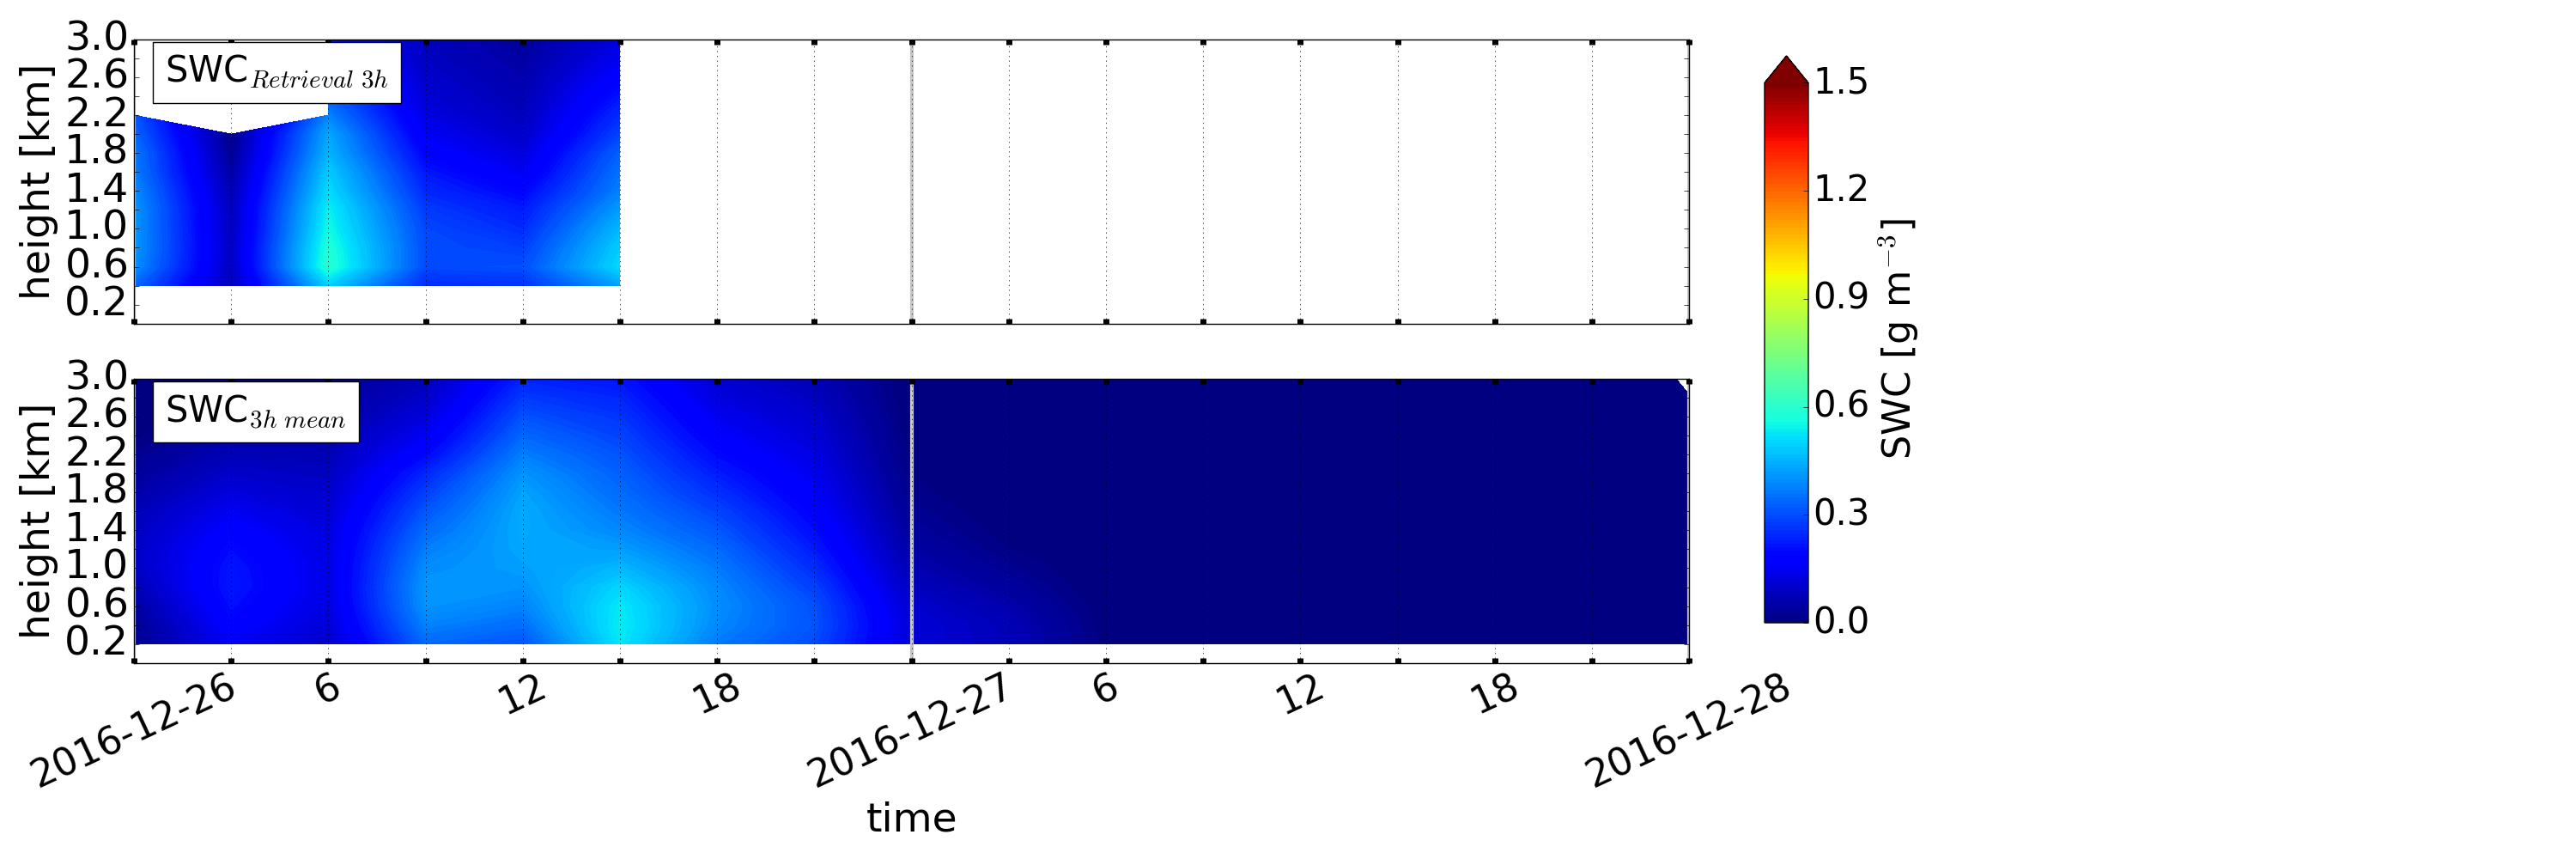
\includegraphics[trim={0.cm 0.8cm 19.cm 0.5cm},clip,width=0.9\textwidth]{./fig_vert_SWC_3h/20161226}
		\caption{}\label{fig:SWC3h:26}
    \end{subfigure}
    \caption{Initialisation \SIlist{23;25;26}{\dec} \SI{0}{\UTC}. 
    (\protect\subref{fig:SWC:ret_23}, \protect\subref{fig:SWC:ret_25}, \protect\subref{fig:SWC:ret_26}) Upper panel: MRR reflectivity for \SI{48}{\hour}, lower panel minutely retrieved SWC. 
    (\protect\subref{fig:SWC_EM:23}, \protect\subref{fig:SWC_EM:25}, \protect\subref{fig:SWC_EM:26}) Upper panel: hourly averaged retrieved SWC, lower panel instantaneous hourly averaged forecast of all ensemble member SWC, neglecting missing values. 
    (\protect\subref{fig:SWC3h:23}, \protect\subref{fig:SWC3h:25}, \protect\subref{fig:SWC3h:26}) Upper panel three hourly averaged retrieved SWC, lower panel instantaneous three hourly averaged forecast of all ensemble member SWC.   }\label{fig:ret:SWC}
\end{figure}
%%%%%%%%%%%%%%%%%%%%%%%%%%%%%%%%%%%%%%%%%%%%%%%%%%%%%%%%%%%%%%%%%%%%%%%%%
\\
It also shows, that the deterministic forecast has for \SIlist{25;26}{\dec} higher SWC predicted than the other ensemble members. This might have led to overestimation at the surface on \SI{26}{\dec}, where the deterministic forecast indicates higher values than the perturbed members, it lies at the upper end of all members (\Cref{fig:}). 
\\
The \SI{25}{\dec} showed patterns of liquid precipitation (\Cref{fig:res:obs_masc}) with warm temperatures (\Cref{fig:res:sfc_temp25}) and high reflectivites (\Cref{fig:ret:refl25}) between \SIrange{12}{21}{\UTC}. To see if liquid precipitation was forecasted, the liquid values given in MEPS are summed. \Cref{fig:LWC:24} and \subref{fig:LWC:25} show that initialisations at either \SI{24}{\dec} or \SI{25}{\dec} predict liquid precipitation. 
Positive temperatures were forecasted between \SIrange{12}{21}{\UTC} (\Cref{fig:res:sfc_temp25}) this follows that an interaction between the vertical and surface exists, following to predict the liquid layer correctly. 
High reflectivity values in \Cref{fig:ret:refl25} are present around \SI{18}{\UTC} with layer thickness up to \SI{1.2}{\km}. \Cref{fig:LWC:24} or \subref{fig:LWC:25} show also a narrow thickness up to \SI{800}{\metre}. 
%%%%%%% image liquid forecast 25 %%%%%%%%%%%%%%%%
\begin{figure}[t]
	\centering
    \begin{subfigure}[b]{\textwidth}
    	\centering
        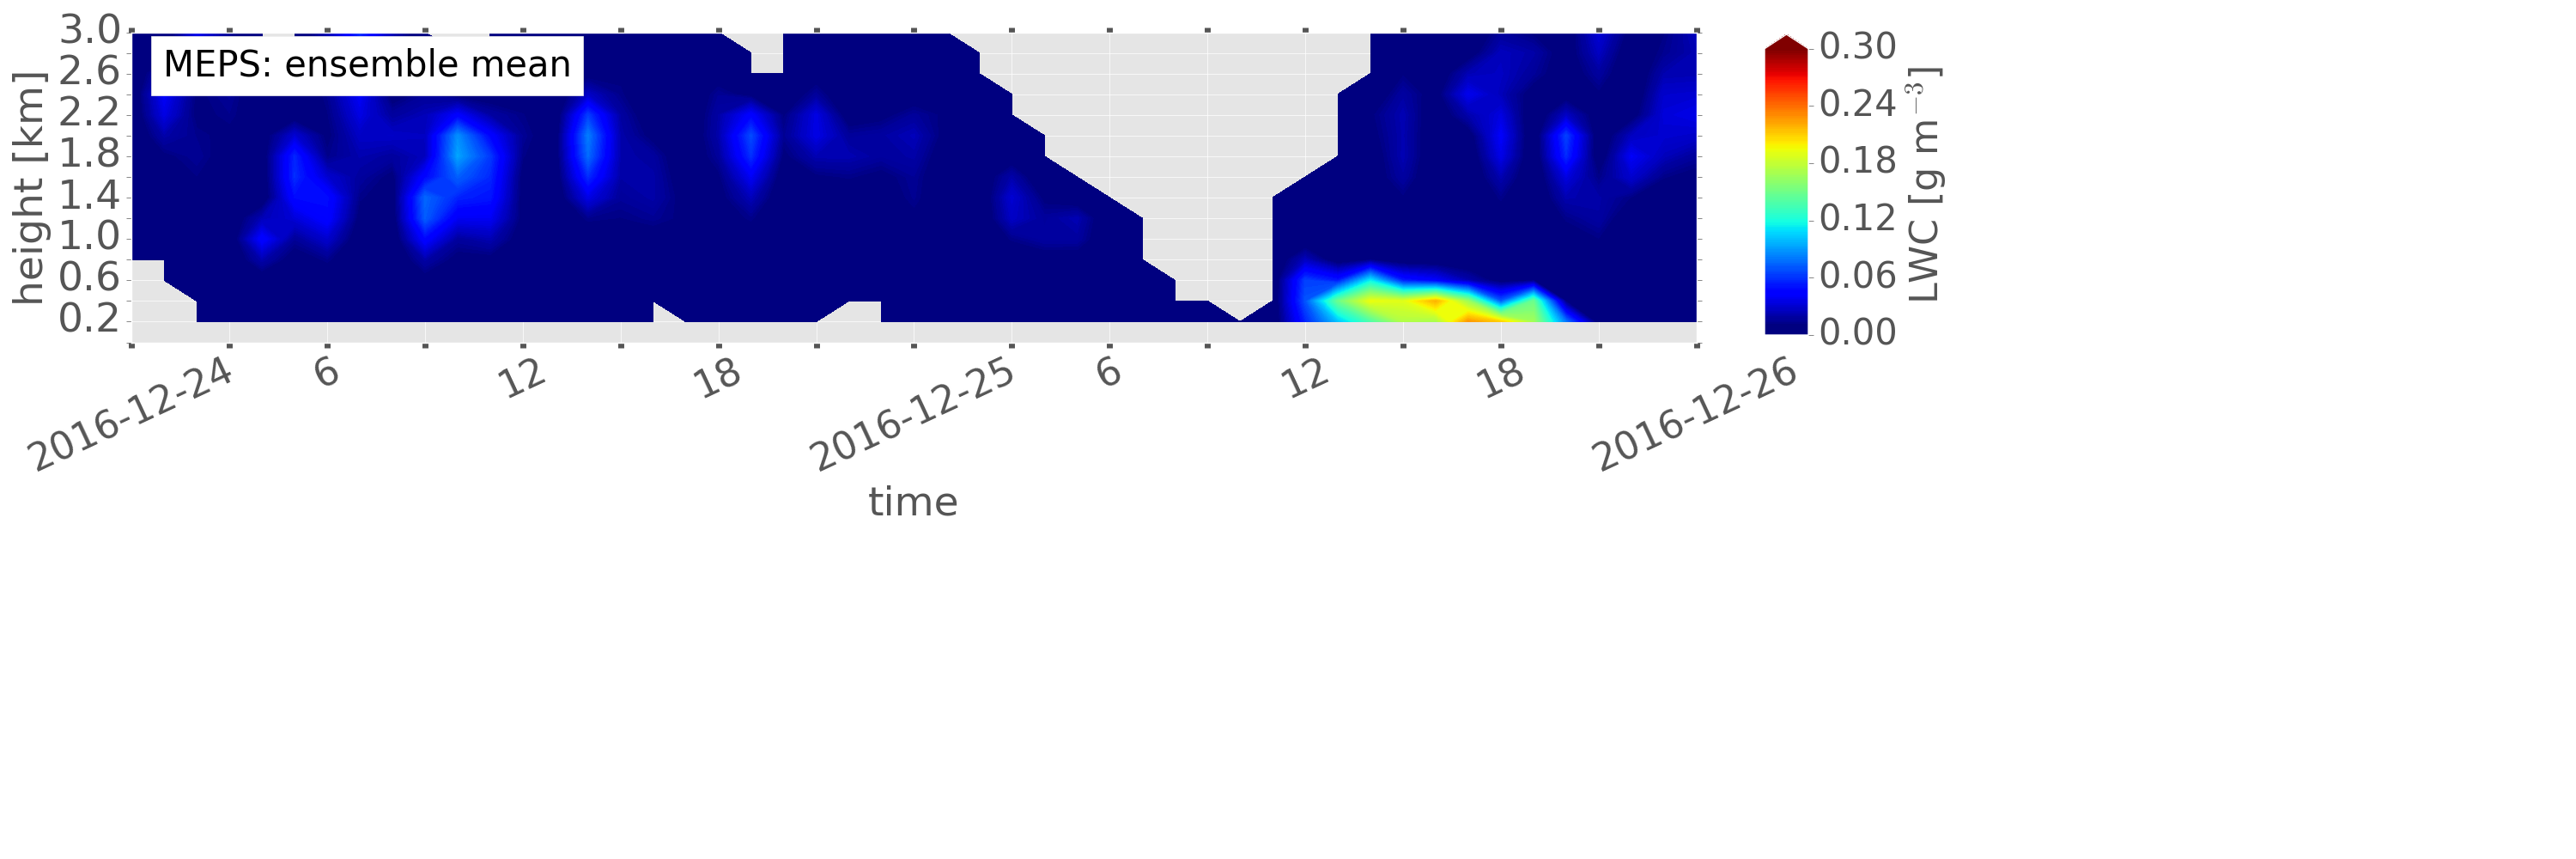
\includegraphics[trim={0.cm 1.9cm 26.5cm 0.4cm},clip,width=\textwidth]{./fig_vert_LWC_EM/20161224}
        \caption{}\label{fig:LWC:24}
    \end{subfigure}
    \begin{subfigure}[b]{\textwidth}
   		\centering
        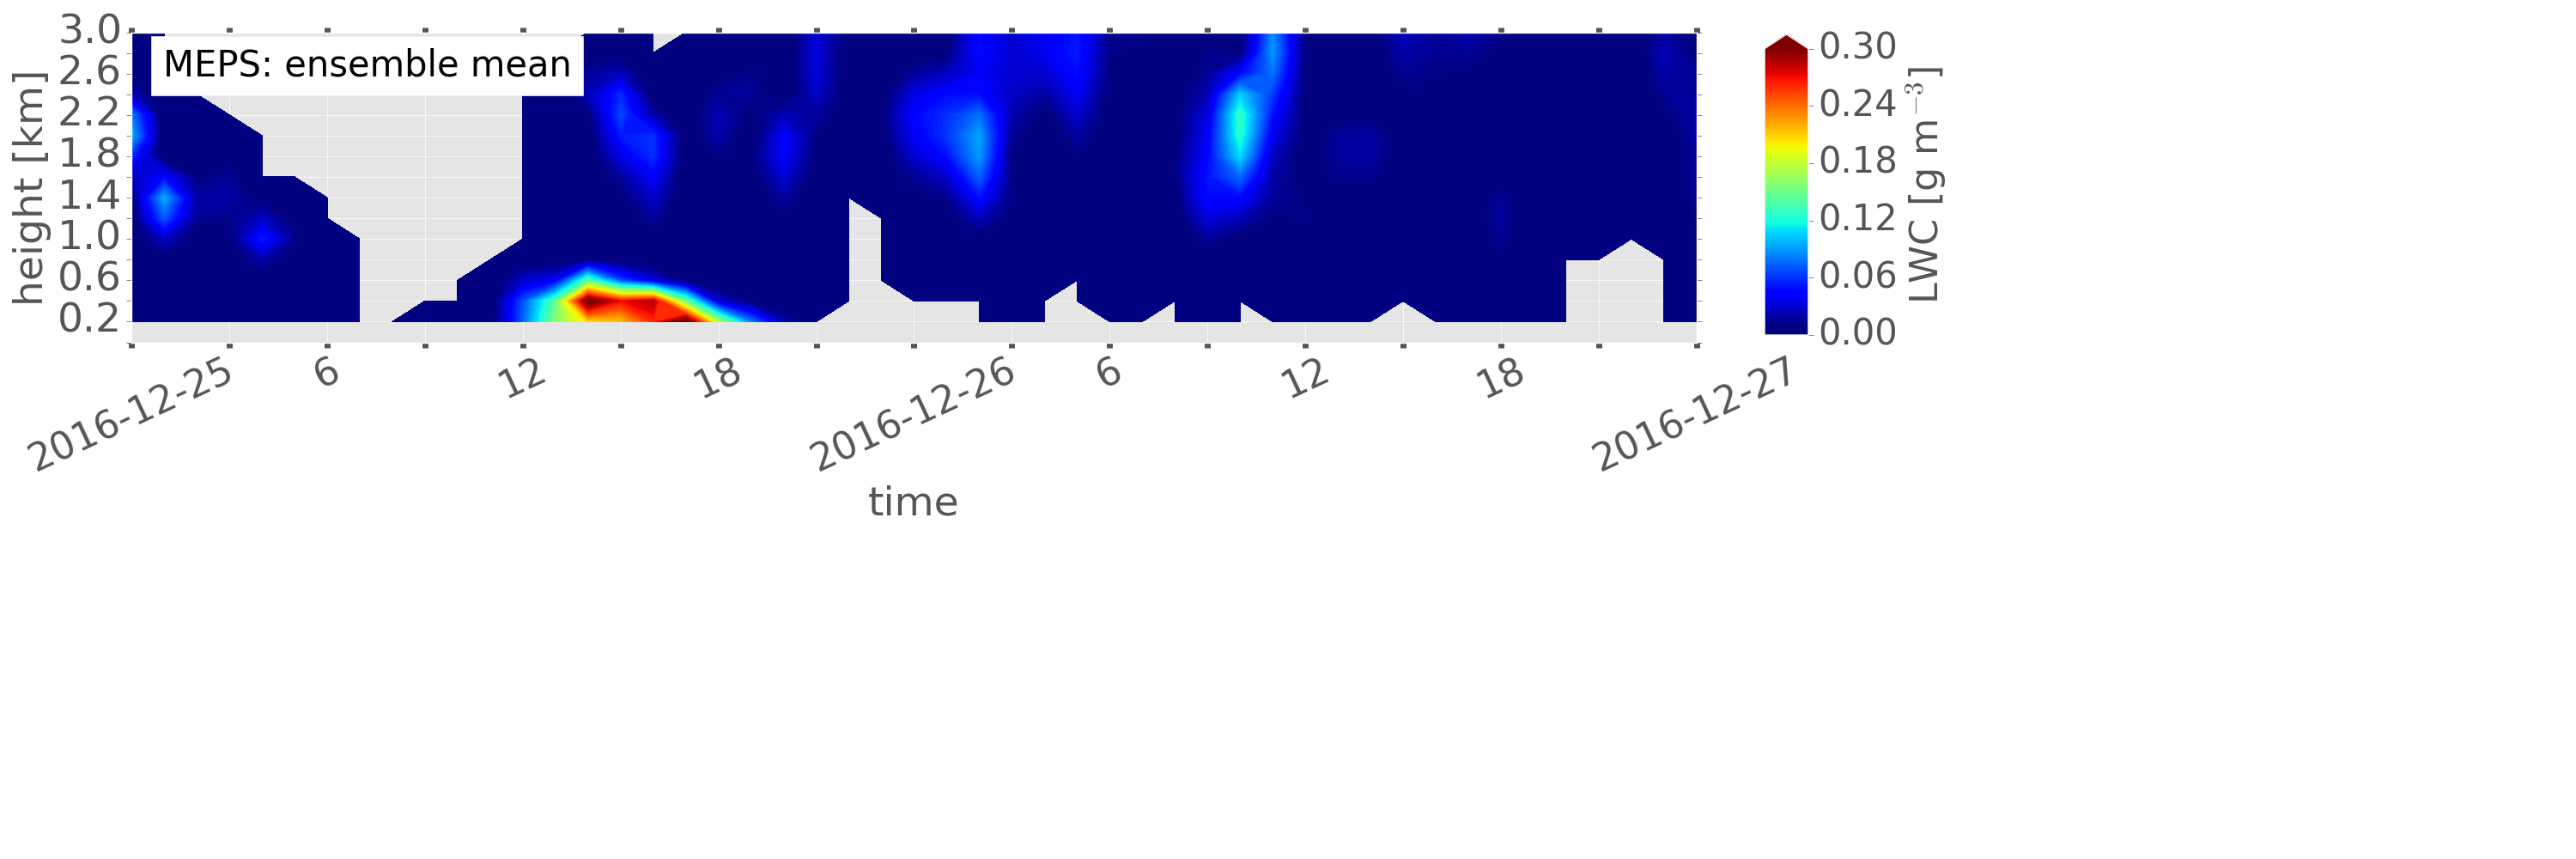
\includegraphics[trim={0.cm 1.9cm 26.5cm 0.4cm},clip,width=\textwidth]{./fig_vert_LWC_EM/20161225}
        \caption{}\label{fig:LWC:25}
    \end{subfigure}
    \caption{Upper panel: 200m hourly averaged LWC forecast from MEPS with all ensemble members, neglecting missing values.
Lower panel: LWP from MEPS, initialised at \SI{0}{\UTC}. Black line represents the deterministic
forecast, the doted blue line the ensemble mean and the grey lines the nine perturbed
members.}\label{fig:res:obs_masc}
\end{figure}
%%%%%%%%%%%%%%%%%%%%%%%%%%%%%%%%%%%%%%%%%%%%%%
\\
It was already shown, that the regional model MEPS is able to predict large scale phenomena correctly for the surface even when the extreme storm gets more intense. The vertical shows the same accuracy for passages of fronts, occlusion and warm sectors, related to a low pressure system.


